\documentclass[a4paper,12pt,oneside,final]{report}
\usepackage[pdftex]{graphicx}
\usepackage{amssymb}
\usepackage{epstopdf}
\usepackage[utf8]{inputenc}
\usepackage{titlesec}
\usepackage[titletoc]{appendix}
\titleformat{\chapter}[hang]{\bf\Huge}{\thechapter}{1cm}{}

\usepackage[colorlinks=true]{hyperref}
\hypersetup{urlcolor=blue,linkcolor=black,citecolor=black,colorlinks=true}
\bibliographystyle{plain}

\pagestyle{plain}
% -------------------- this stuff for code --------------------

\usepackage{anysize}
\marginsize{30mm}{30mm}{20mm}{20mm}

\newenvironment{formal}{%
  \def\FrameCommand{%
    \hspace{1pt}%
    {\color{blue}\vrule width 2pt}%
    {\color{formalshade}\vrule width 4pt}%
    \colorbox{formalshade}%
  }%
  \MakeFramed{\advance\hsize-\width\FrameRestore}%
  \noindent\hspace{-4.55pt}% disable indenting first paragraph
  \begin{adjustwidth}{}{7pt}%
  \vspace{2pt}\vspace{2pt}%
}
{%
  \vspace{2pt}\end{adjustwidth}\endMakeFramed%
}

\newenvironment{changemargin}[2]{\begin{list}{}{%
\setlength{\topsep}{0pt}%
\setlength{\leftmargin}{0pt}%
\setlength{\rightmargin}{0pt}%
\setlength{\listparindent}{\parindent}%
\setlength{\itemindent}{\parindent}%
\setlength{\parsep}{0pt plus 1pt}%
\addtolength{\leftmargin}{#1}%
\addtolength{\rightmargin}{#2}%
}\item }{\end{list}}

\usepackage{color}
\usepackage{dsfont}
\usepackage[bitstream-charter]{mathdesign}
\usepackage[scaled]{helvet}
\usepackage{inconsolata}


\definecolor{colKeys}{rgb}{0,0,0.9} 
\definecolor{colIdentifier}{rgb}{0,0,0} 
\definecolor{colString}{rgb}{0.7,0,0} 
\definecolor{colComments}{rgb}{0,0.6,0} 
\usepackage{listings}
\lstset{
  stringstyle=\color{colString},
  keywordstyle=\color{colKeys},
  identifierstyle=\color{colIdentifier},
  commentstyle=\color{colComments},
  numbers=left,
  tabsize=4,
  frame=single,
  breaklines=true,
  basicstyle=\small\ttfamily,
  numberstyle=\tiny\ttfamily,
  framexleftmargin=0mm,
  xleftmargin=7mm,
  xrightmargin=7mm,
  frameround={tttt},
  captionpos=b
}

\usepackage{mathtools}
\usepackage{amsthm}
\newtheorem{definition}{Definition}
\newtheorem{theorem}{Theorem}
\DeclareMathOperator*{\argmin}{ArgMin\ }
\DeclareMathOperator*{\argmax}{ArgMax\ }

\usepackage{algorithm}
\usepackage{algorithmic}

\usepackage[usenames,dvipsnames]{xcolor}
\makeatletter
\DeclareRobustCommand{\em}{%
  \@nomath\em \if b\expandafter\@car\f@series\@nil
  \normalfont \else \bfseries \fi}
\makeatother

%% Headers and footers
\usepackage{fancyhdr}
\usepackage[section]{placeins}
\pagestyle{fancy}
\fancyhf{}
\addtolength{\headwidth}{30pt}
\addtolength{\headwidth}{30pt}
\renewcommand{\headrulewidth}{0.4pt} % thickness of the header line
\renewcommand{\footrulewidth}{0.4pt} % thickness of the footer line
\renewcommand{\chaptermark}[1]{\markboth{#1}{#1}} % chapter name
\renewcommand{\sectionmark}[1]{\markright{\thesection\ #1}}  % section name
\lhead[\fancyplain{}{\bf\thepage}]{\fancyplain{}{\bf\rightmark}} % display header
\rhead[\fancyplain{}{\bf\leftmark}]{\fancyplain{}{}} % display header
\fancyfoot[C]{\bf\thepage} % display footer (page number)
\fancyfoot[R]{\bf\today} % display footer (date)
\fancypagestyle{plain}{ 
	\fancyhead{} \renewcommand{\headrulewidth}{0pt}
}
\newcommand{\clearemptydoublepage}{\newpage{\pagestyle{plain}\cleardoublepage}}

\usepackage[T1]{fontenc}
\usepackage{enumerate}
\usepackage{afterpage,lastpage,fancyhdr}
\usepackage[includeheadfoot,margin=2.5cm]{geometry}
\geometry{letterpaper}                   % ... or a4paper or a5paper or ... 

\DeclareGraphicsRule{.tif}{png}{.png}{`convert #1 `dirname #1`/`basename #1 .tif`.png}

\makeatletter \def\thickhrulefill{\leavevmode \leaders \hrule height 1pt\hfill
\kern \z@} \renewcommand{\maketitle}{
    \begin{titlepage}
    \let\footnotesize\small \let\footnoterule\relax \parindent \z@ \reset@font
    \null\vfil
    \vspace{-20mm}
    \begin{center}
    {\small \scshape Imperial College London \\ Department of Computing}
    \end{center}
    \vspace{0.5cm}
	\begin{minipage}{\textwidth}
		\vspace{1cm}
		\noindent\rule[0ex]{\textwidth}{4pt} \\
		\flushright
		\center
		\@title
		\\ \vspace{4mm}
		\noindent\rule[0ex]{\textwidth}{4pt} \\
	\end{minipage}
	\vspace{1.5cm}
	\begin{minipage}{\textwidth}
		\flushright
		{\bfseries}
		\vspace{7mm}
		\center
		\@author.\\
	\end{minipage}
	\vspace{0.5cm}
	\begin{center}
		
\includegraphics[width=70mm,]{logo_imperial_college_london.png}
	\end{center}
	\vspace{\stretch{1}}
	\vspace{50mm}
		\flushleft
		{\bfseries}
		Module leader \& Lecturer: Dr Maja \textsc{Pantic}. \\
		{\small \scshape \@date }.
		\vspace{0.1cm}
		\rule{\linewidth}{.5pt}
  \end{titlepage}
  \setcounter{footnote}{1}
  \setcounter{page}{2}
}


\author{
    Sedef Ozlen (so512, s5) \\ 
    Paul Gribelyuk (pg1312, a5) \\
    Jean Kossaifi (jk712, a5) \\ 
    Romain Brault (rb812, a5)
}
\makeatother
\title{\Huge Machine Learning \\ Case Based Reasoning \\ Coursework 4}
\date{\today}


\usepackage{amsmath}
\begin{document}
\maketitle
\tableofcontents
\listoffigures

\chapter{Introduction}
The purpose of the Case-Based Reasoning was to gain familiarity with the classification algorithm based on a similarity measure and a database of examples to compare new data with.  The critical component was to implement an intelligent structure to store and access the data when performing classification.  We found that the algorithm forces a tradeoff between performance and accuracy since clustering, the solution we chose, allows us to narrow down the set of cases to search through at the cost of misclassifying a small percentage of data.  
Through this module, we learned that \emph{lazy learning} can be applied to infer information by blurring the training and the classification stage of the machine learning process.  By continuously adding new data to the database of cases, we are able to improve the classification rate as the machine is presented with previously unseen examples.

\chapter{Implementation of CBR}
\paragraph{}
The first stage of CBR is to create an initial database of cases (case base).  We do this with the following MATLAB call:
\begin{changemargin}{-5mm}{-5mm}
\begin{lstlisting}[language=Matlab, frame=single]
case_base = CBRinit(x, y)
\end{lstlisting}
\end{changemargin}
where \verb+x+ and \verb+y+ are initial cases with their correct classifications, respectively.  We split this data according to their class, creating a bucket within the case base in the following way:
\begin{changemargin}{-5mm}{-5mm}
\begin{lstlisting}[language=Matlab, frame=single]
CBR.base{i}.vector = CaseStr.empty;
CBR.base{i}.count = 0;
CBR.base{i}.meanVec = zeros(1,size(x,2));
\end{lstlisting}
\end{changemargin}
where the \verb+vector+ field contains a list of \verb+CaseStr+ objects, the \verb+count+ field is the number of cases in that cluster, and the \verb+meanVec+ field stores the average action unit (AU) example associated with that cluster.  
We represent a case (\verb+CaseStr+ in our code), as an object with the properties:
\begin{changemargin}{-5mm}{-5mm}
\begin{lstlisting}[language=Matlab, frame=single]
properties
    activeAU;
    solution;
    timesRetrieved = 0;
end
\end{lstlisting}
\end{changemargin}
storing the indices of the active AUs, the class associated with that case, and the typicality of the case.

\paragraph{}
Our \verb+retrieve+ algorithm 
\paragraph{}
What to do when adding an example which already exists in the case base?  We chose to take into account examples which already exist in the case base by modifying the mean but not adding the case to the database.  This give that AU array greater weight without unnecessarily complicating the implementation.

Similarity measure 1: number of common active Action Units: if Case1 has some active action units $a^{1}_{i}$ and Case 2 has some other active action units $a^{2}_{i}$.  Then the similarity measure will be the size of the set $\{ a^{1}_{i} = a^{2}_{i}\}$

Similarity measure 2: difference in the number of active action units.  The similarity measure is $|\{a^{1}_{i}\}| - |\{a^{2}_{i}\}|$
\paragraph{}

\chapter{}
\paragraph{}
\section{}
\paragraph{} 
\begin{changemargin}{-5mm}{-5mm}
\begin{lstlisting}[language=Matlab, frame=single]
sample MATLAB code
\end{lstlisting}
\end{changemargin}
\label{ch:build}
\begin{itemize}
\item {\bf \textit{item 1} } sample itemized list
\item {\bf \textit{item 2} } sample itemized list
\end{itemize}

\paragraph{}
\paragraph{}
\section{Some section}
\begin{changemargin}{-5mm}{-5mm}
\begin{lstlisting}[language=Matlab, frame=single]
more MATLAB code
\end{lstlisting}
\end{changemargin}

\section{Some section heading}
\paragraph{}
\chapter{Sampel Chapter}
\paragraph{}
\section{Sample Section}
\subsection{Sample Subsection}
\paragraph{}
\paragraph{}
\paragraph{}
\paragraph{}
\paragraph{}
\section{Another section}
\section{Yet another section}

\paragraph{}

\begin{algorithm}[H]
     \caption{\small Double cross validation}
     \label{alg:double_cross_val} 
     \begin{algorithmic}
       \STATE \begin{tabular}{@{\hspace{0cm}}p{1.4cm}l}
       \textbf{Parameters}  & $(x, y)$ : observation matrix and the vector of associated labels.\\
           & $C$ : hyper-parameters vector\\
           & $K_{ext}$ : number of folds for the outer loop\\
           & $K_{int}$ : number of folds for the inner loop\\
       \end{tabular}
       \STATE $KFold_{ext} \leftarrow \text{ divide x into } K_{ext} \text{ folds}$\\
     \FOR{i \textbf{from} 1 \TO $K_{ext}$}
         \STATE $\text{valid}_{ext}[i] \leftarrow 1 \text{ bloc of } KFold_{ext}$
         \STATE $\text{train}_{ext}[i] \leftarrow \text{ the other blocks of } KFold_{ext}$
         \STATE $KFold_{int} \leftarrow \text{ divide train}_{ext}[i] \text{ into } K_{int} \text{ folds}$\\
         \FOR{j \textbf{from} 1 \TO $K_{int}$}
            \STATE $\text{valid}_{int}[j] \leftarrow 1 \text{ bloc of } KFold_{int}$
            \STATE $\text{train}_{int}[j] \leftarrow \text{ the other blocks of } KFold_{int}$
            \FOR{k \textbf{from} 1 \TO size(C)}
               \STATE $\text{model}_{int}$[j, k] $\leftarrow$ fit-algorithm($\text{train}_{int}[j]$)
               \STATE $\text{error}_{int}$[j, k] $\leftarrow$ compute-error($\text{model}_{int}[j]$, $\text{valid}_{int}[j]$))
            \ENDFOR
         \ENDFOR
         \STATE $\text{error}_{int}$[i]$ \leftarrow  \text{mean}_j( \text{error}_{int}$[j,k])
         \STATE $\text{C}_{opt}$[i]$     \leftarrow  \text{min}( \text{error}_{int}$[i])
         \STATE $\text{model}_{ext}$[i]$ \leftarrow  \text{fit-algorithm}( \text{train}_{ext}$[i], $\text{C}_{opt}$[i])
         \STATE $\text{error}_{ext}$[i]$ \leftarrow  \text{compute-error}( \text{model}_{ext}$[i], $\text{valid}_{ext}$[i])
     \ENDFOR 
     \STATE $\text{error}_{test} \leftarrow  \text{mean}_i( \text{error}_{ext}$[i])
     \RETURN $\text{error}_{test}$ 
     \end{algorithmic}
   \end{algorithm}


\begin{figure}[!h]
\begin{changemargin}{-20mm}{-20mm}
\center
%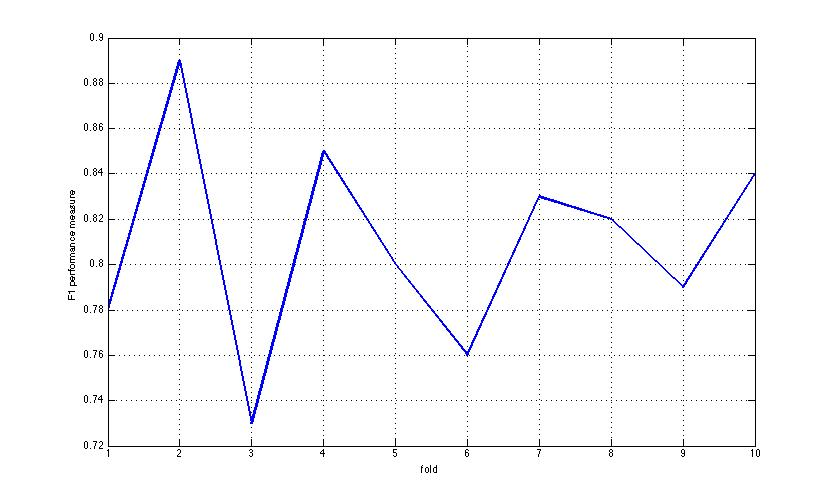
\includegraphics[scale=0.5]{single_perf.jpg}
\caption{A figure caption}
\end{changemargin}
\end{figure}

\paragraph{}
\chapter{Conclusion}
\paragraph{}

\bibliographystyle{alpha}
\bibliography{biblio.bib}

\begin{appendices}

\end{appendices}

\end{document}  
